\chapter{Tools from the sky}\label{ch:skytools}

\section{Why cosmology's tools fit the cell}

The cosmic horizon and the cell are two places in IAM: surfaces where records are written at a temperature (Part~\ref{part:1}). In each, the record is
read through an instrument that drifts, under foregrounds far brighter than the signal, and in each there is only one specimen to read: one sky,
one person's cells. Cosmology met that problem first. It reads temperature differences of one part in $10^5$ about 2.7255~K~\cite{Fixsen2009}, under dust and
synchrotron emission from our own galaxy, with detectors whose gain changes by the hour, and it has no second universe to repeat the
measurement on. The tools it built for that are the tools this chapter carries into the methylome. Some are algorithms; the more important ones
are a discipline against fooling oneself.
Cosmology was forced into this precision by its data: an accelerating expansion, and a microwave background that had to be measured to
fractions of a per cent. In meeting that demand it built Markov-chain Monte Carlo for many-parameter models, convergence diagnostics that
say when a result can be trusted~\cite{Gelman1992}, and a culture of stating a prediction before the data arrive. Biology was rarely forced
to build the equivalent. We are not borrowing cosmology's vocabulary. We are borrowing its measuring equipment, which it spent decades
building, and pointing it at the cell.

\section{How the CMB is read}

A CMB experiment goes from raw detector samples to physics in fixed steps: calibrate the time-ordered data and cut glitches; make a map on a sphere;
remove the foregrounds by component separation, using that each emitter has its own spectrum; measure what is left against noise maps made from
split halves of the data; and only then compute statistics (power spectra, higher-order shapes, isotropy tests), with every test fixed before
the answer is seen. Figure~\ref{fig:cmbcell}a is that residual for one simulated Planck sky.
The signal itself was first found as an excess in a noise budget: 3.3~K above the components of the Echo receiver in 1961, and 3.5~K in
Penzias and Wilson's horn in 1965, identified that year as the radiation of the early universe~\cite{Ohm1961,PenziasWilson1965,Dicke1965,Wilson1979}.
\observed{} It had been present and detectable the whole time; what was missing was a precise enough instrument and knowing what to look for.
A cell's departure from its healthy reading is the same kind of signal: small, under a brighter foreground, and visible only to an
instrument built to see it. \analogy

\begin{figure}[htbp]\centering
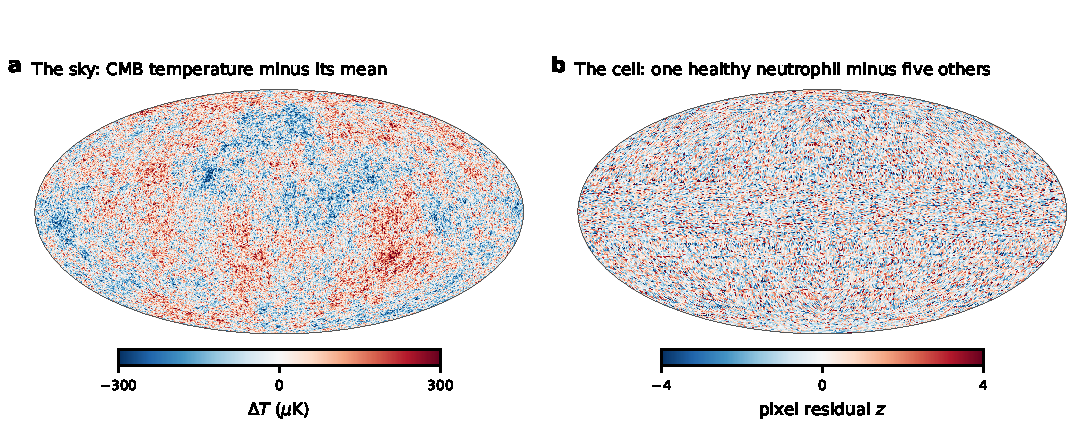
\includegraphics[width=\textwidth]{figures/part4/fig_sky_cmb_vs_neutrophil.pdf}
\caption{Same projection, same kind of quantity. (a) A sky drawn from the Planck 2018 best-fit temperature power spectrum~\cite{Planck2018VI} (CAMB 2.0.4~\cite{Lewis2000CAMB},
$H_0=67.36$, $\Omega_bh^2=0.02237$, $\Omega_ch^2=0.1200$, $\tau=0.0544$, $A_s=2.100\times10^{-9}$, $n_s=0.9649$; HEALPix~\cite{Gorski2005} $N_{\rm side}=256$,
seed 42): temperature minus its mean. (b) One healthy neutrophil array (GSM2998021) read against the other five physical arrays of the healthy
reference: residual $z$ at 454,674 reference sites, placed in genome order on HEALPix rings ($N_{\rm side}=64$) and summed per pixel as
$\sum z/\sqrt n$. The CMB's structure is the signal; a healthy cell's sky is quiet by construction, so any structure in it is the finding.}\label{fig:cmbcell}
\end{figure}

The cell's chain follows the same steps. The difference that matters is the last column of the CMB: its structure is the
signal. In the cell the reference is the same cell type in healthy people, so a healthy specimen reads a quiet sky and the signal is the
departure.

\begin{center}\small
\begin{tabular}{@{}p{0.3\textwidth}p{0.36\textwidth}p{0.26\textwidth}@{}}\toprule
CMB step & methylome step & chain v3 \\\midrule
time-ordered data, glitch cuts & IDAT intensities, control probes, detection masking & Stages 0--1 \\
gain and bandpass calibration & dye bias, probe types, bisulfite conversion; same-run tare & Stages 1 and T \\
map-making & intensity to $\beta$ & Stage 1 \\
component separation & composition of the specimen (8 blood groups) & Stage A \\
residual map & $z$ at each identity site against the healthy reference & Stage M \\
monopole & Met-A, the mean over identity sites & Stage M \\
clustering of the residual & C-score & Stage MC \\
null tests on split data & held-out reference arrays, repeat specimens & development \\\bottomrule
\end{tabular}
\end{center}

\section{Putting the genome on a sphere}

HEALPix~\cite{Gorski2005} divides the sphere into $12N_{\rm side}^2$ pixels of equal area, arranged on rings of constant latitude. The chain lays CpGs on it in
genome order, chromosome 1 to chromosome Y and by position within each, filling the pixels ring by ring from the north pole
(Figure~\ref{fig:genomesphere}). On EPIC this places 865,873 CpGs on 49,152 pixels ($N_{\rm side}=64$), 17.6 per pixel; the atlas map uses
$N_{\rm side}=128$ for its 483,092 CpGs, 2.5 per pixel. \calc

\begin{figure}[htbp]\centering
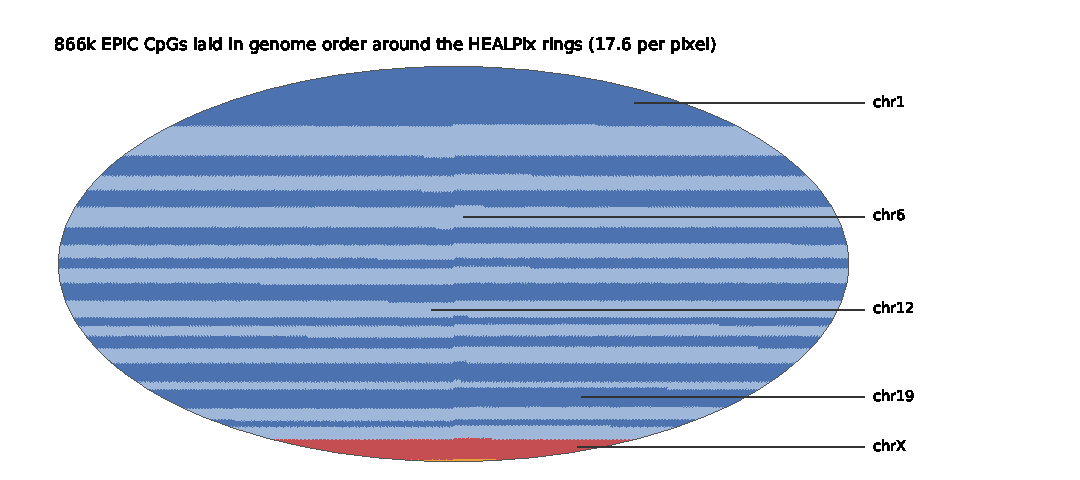
\includegraphics[width=\textwidth]{figures/part4/fig_sky_genome_on_sphere.pdf}
\caption{The genome on the sphere. Chromosomes alternate in two blues, chrX red, chrY orange (the thin cap at the south pole). Each band is one
chromosome; its width is its number of EPIC CpGs.}\label{fig:genomesphere}
\end{figure}

The layout is a display choice, not physics. Neighbours along a ring are genomic neighbours; neighbours above and below are millions of bases
apart. Everything quantitative in the chain therefore works along the genome itself, and the sphere is how a person sees it: a quiet sky, a
streak along a ring (one genomic region), a band (one chromosome).

\paragraph{Is the sphere needed?} For the measurement, no: the residual is a sequence along the genome, and every statistic in the chain
is computed along it. For the toolkit it is convenient, because needlets, harmonic decompositions and masked-sky spectra are written for
the sphere. For a person reading one specimen it is probably the wrong picture, since the sphere carries no chromosome coordinates. A
per-chromosome linear track, the format of every genome browser, or a Hilbert-curve layout, a space-filling curve already used to show
genomic data~\cite{Anders2009}, keeps neighbouring sites together and stays rectangular. The intended display is both, drawn from one
residual so that the two cannot disagree. \openprob{} (not built)

\section{Reading a cell's sky}

At each site $i$ the residual is
\begin{equation}
  z_i=\frac{H(\beta_i)-\overline{H}_i}{s_i},
\end{equation}
where $\overline{H}_i$ is the mean of $H(\beta)$ over the healthy reference arrays and $s_i$ their spread, shrunk toward the pooled spread as in
the chain. Two numbers summarise the sky. Met-A is its monopole, the mean of $H(\beta)$ over the 6,000 identity sites divided by the healthy
reference. The C-score asks whether the departures sit together along the genome: take $z$ in genome order, average it in blocks of 50 sites,
and compare the variance of the block means (times 50) with the variance of $z$. Independent scatter gives 1; a pattern in which every 50-site
block moves as one gives 50. Divided by the healthy baseline 1.1104, the healthy arrays read 0.70--1.23 and the far end is 45 (Chapter~\ref{ch:cscore}). \derived{} (construction) \calibrated{} (baseline)

Figure~\ref{fig:whatitsees} reads the six physical healthy arrays, each against the other five, and the same arrays with known damage:
% generated by make_skytools_tables.py; do not edit by hand
\begin{center}\small
\begin{tabular}{@{}lcc@{}}\toprule
specimen & Met-A & C-score \\\midrule
healthy (6 arrays) & 0.993--1.008 & 0.71--1.23 \\
2\,\% blur everywhere (6 arrays) & 1.096--1.110 & 0.78--1.23 \\
5\,\% blur, 10 regions (6 arrays) & 1.005--1.020 & 12.53--15.70 \\
\bottomrule\end{tabular}
\end{center}

\measured{} The table's healthy C-score, 0.71--1.23, comes from the sky-map construction, whose lowest healthy array reads 0.705; the chain's
own reading of the same six arrays is 0.70--1.23 (lowest 0.699), the range quoted above. Damage spread over every site moves Met-A by about 0.1 and leaves the C-score where it was. The same damage concentrated in ten
regions holding 5\,\% of the sites leaves Met-A inside Normal (0.95--1.05) and raises the C-score to 12.5--15.7. Met-A and the C-score measure
different things; a reading needs both (Figure~\ref{fig:cunrolled}).

\begin{figure}[htbp]\centering
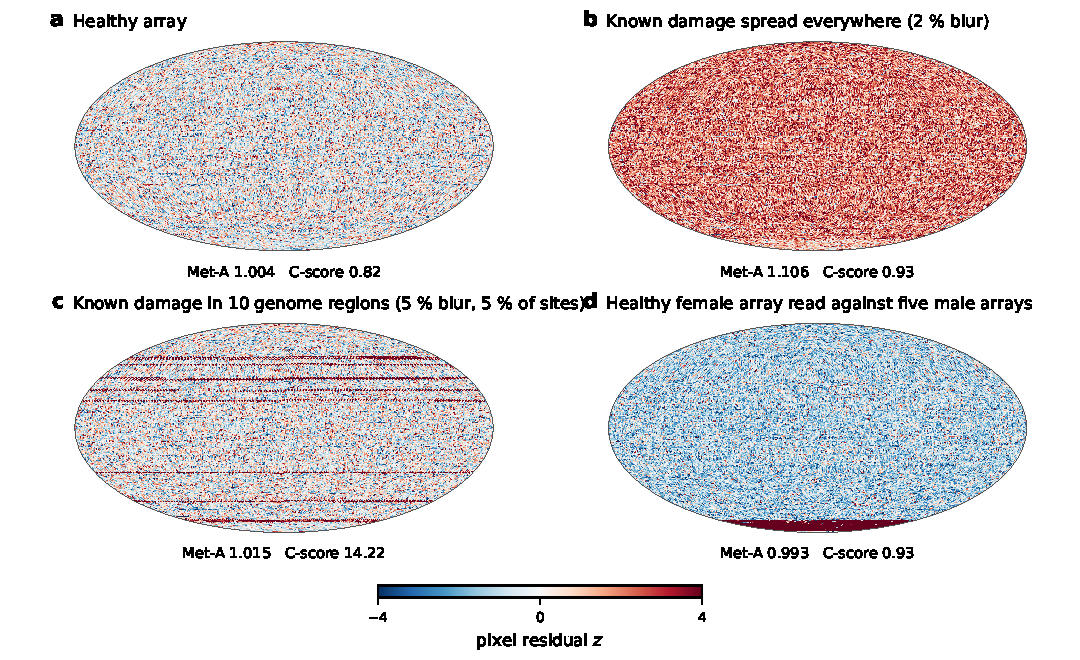
\includegraphics[width=\textwidth]{figures/part4/fig_sky_what_it_sees.pdf}
\caption{What the sky sees. (a) A healthy array. (b) The same array with 2\,\% blur toward $\beta=0.5$ at every site. (c) 5\,\% blur inside ten
contiguous genomic regions (5\,\% of sites): streaks along rings. (d) The one female array of the reference read against the five male arrays:
chrX lights up at the south pole. Met-A and C-score under each map are the chain's readings at the 6,000 identity sites (for c, the same
construction applied to the identity sites).}\label{fig:whatitsees}
\end{figure}

\begin{figure}[htbp]\centering
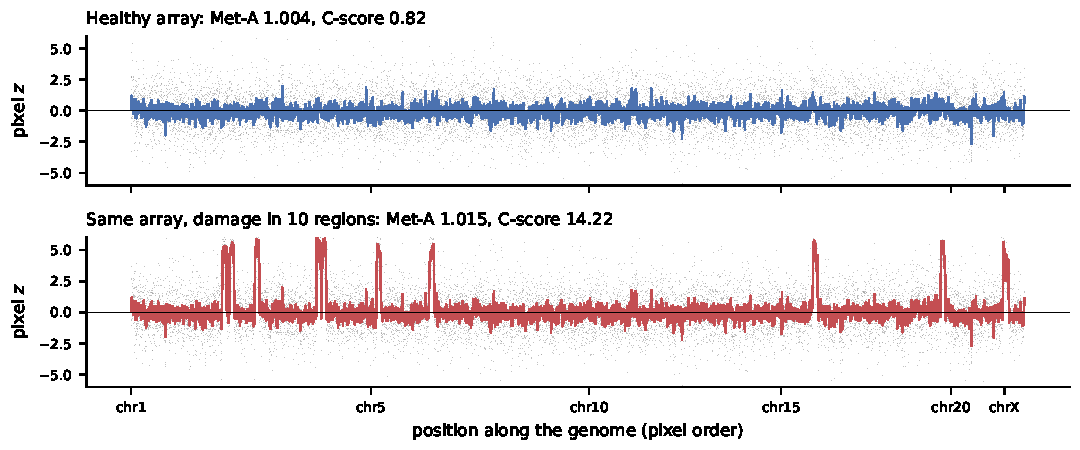
\includegraphics[width=\textwidth]{figures/part4/fig_sky_cscore_unrolled.pdf}
\caption{The C-score, unrolled. Pixel $z$ along the genome (grey points) with a 25-pixel running mean, for a healthy array and the same array
with damage in ten regions. Each damaged region is a run of consecutive sites; the block average catches it while the mean over all sites
barely moves.}\label{fig:cunrolled}
\end{figure}

\paragraph{The sky found the X chromosome.} Panel~\ref{fig:whatitsees}d was not planned as a test. One of the six reference arrays reads as female: 40\,\% of her chrX sites read between $\beta=0.3$ and 0.7, against 8\,\% in the other five, and only 121 of her chrY probes are
detected, against about 540 in the others. \measured{} Read against five male arrays, X inactivation is a foreground the size of a galaxy plane. It
does not reach Met-A: the 32 identity sites on chrX read the same $\beta$ on her array and on the five male arrays, because
the site rule required agreement across all six arrays. \measured{} The lesson is the CMB's: a whole-array map needs a sex mask, or a reference of
the same sex, before its structure means anything. \openprob

\section{The methylome's power spectrum}

The CMB's first statistic is its angular power spectrum: how strongly two points of the sky agree as a function of the angle between them.
The genome's counterpart is the correlation of methylation between two CpGs as a function of the number of bases between them, $C(d)$,
measured inside one specimen. Figure~\ref{fig:cd}a is $C(d)$ for each of the six healthy neutrophil arrays. \measured{} Neighbouring CpGs
agree almost completely (0.97 at 10--18~bp); agreement halves just below 1~kb, falls to 0.32 at 1--1.8~kb and to 0.05 at 3--6~kb, and a weak tail
remains out to megabases. The six arrays give the same curve to the second decimal (0.321--0.327 at 1~kb). Co-methylation that falls with the distance between CpGs
is also seen in bisulfite sequencing~\cite{Eckhardt2006}. At this resolution the curve falls smoothly; it shows no peak at the nucleosome
repeat (about 200~bp), and the array's probe spacing is too coarse to rule one out. A molecule-level $C(d)$ from sequencing reads is the test.

\begin{figure}[htbp]\centering
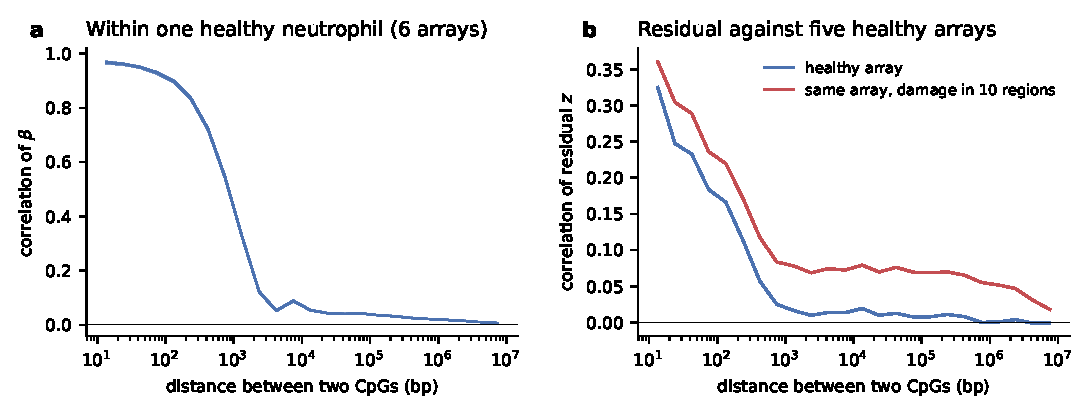
\includegraphics[width=\textwidth]{figures/part4/fig_sky_cd.pdf}
\caption{Genome-distance correlation inside one specimen. (a) $\beta$ at two CpGs on the same chromosome, correlated across all such pairs
(up to 300,000 random pairs per distance bin), for each of the six healthy neutrophil arrays. (b) The residual $z$ of one array read against
the other five: healthy, and with 5\,\% blur in ten regions.}\label{fig:cd}
\end{figure}

The residual's $C(d)$ (Figure~\ref{fig:cd}b) is the noise model's check. In a healthy array the residual is correlated over a few hundred
bases, because the probe chemistry and neighbouring CpGs share it, and is uncorrelated beyond 1~kb (0.00--0.02). Regional damage adds a
plateau of 0.05--0.08 from 1~kb out to about a megabase, the size of the damaged regions. \measured{} This is the spectrum the C-score
condenses into one number, and it is the right null for any whole-array map: a healthy map is correlated at short range, so a structure has
to be tested against a genome-shuffled healthy map, not against independent noise.
A Gaussian null would call the healthy baseline a finding every time.

\paragraph{A test the C-score was built for.} Cancer and ageing erode methylation over whole genomic neighbourhoods, the late-replicating
partially methylated domains~\cite{Berman2012,Zhou2018PMD}. If that
erosion is regional in one person's cells, the C-score will rise where Met-A, which averages over all identity sites, barely moves, as the
constructed damage of Figure~\ref{fig:whatitsees}c does. \prediction{} The blood-cancer arrays are the first test, read per person against the
healthy reference of the same cell type.

\paragraph{Isotropy by chromosome arm.} The same per-person map, averaged by chromosome arm, separates a change spread over the whole genome
from one confined to an arm. Tumours often gain or lose whole arms (8q, 17p and others); on an array that shows as a shift in total intensity
and in $\beta$ along the arm. Panel~\ref{fig:whatitsees}d is this test finding the X chromosome. The arm-level map, with a copy-number track
from the same array's intensities beside it, is on the build list.

\section{The map, scored}

Before the chain was built, a CMB analysis pipeline was translated into methylome terms row by row: 79 rows. Table~\ref{tab:map79} scores every row against chain v3. Counts: in use 12; built, not in chain 3; partial 9; calculated 1; measured 1; reserved 3; not built 31; open 1; analogy 10; refused 2; out 4; does not translate 2. \observed

% generated by make_skytools_tables.py (not in this repository; the file is now maintained by hand, see the notes below)
% edited by hand 2026-10-02 (generator not in the repo): the product name removed from rows 33 and 79; row 7 Stage T text
% edited by hand 2026-10-03 (proposal): reference counts, a development number and a commit removed from rows 1, 12, 22, 79
% edited by hand 2026-10-03 (verification pass): light row rules (\rowrule, preamble) between body rows
\newcommand{\mapcounts}{in use 12; built, not in chain 3; partial 9; calculated 1; measured 1; reserved 3; not built 31; open 1; analogy 10; refused 2; out 4; does not translate 2}
\begin{center}\scriptsize
\begin{longtable}{@{}r p{0.21\textwidth} p{0.32\textwidth} p{0.12\textwidth} p{0.18\textwidth}@{}}
\caption{The 79-row CMB-to-methylome map, scored against chain v3 on 2 October 2026.}\label{tab:map79}\\
\toprule \# & CMB tool & counterpart in the cell & status & where \\\midrule\endfirsthead
\toprule \# & CMB tool & counterpart in the cell & status & where \\\midrule\endhead
1 & Spherical-harmonic decomposition & projection of a specimen onto a basis of reference cells & in use & Stage A solves 8 blood groups; the atlas holds the full basis \\ \rowrule
2 & Monopole, dipole, low multipoles & monopole = Met-A (mean over identity sites); sex shows as a chrX patch & in use & Fig. sky-what-it-sees d \\ \rowrule
3 & Cosmic variance & cell-count floor: finite genome copies in a specimen & calculated & Ch. sky; not in the chain; needed for plasma \\ \rowrule
4 & Frequency coverage & more than one mark or assay per cell (5mC, 5hmC; arrays and single molecules) & partial & Met-A (arrays) and IAM-A (single molecules) read one cell two ways \\ \rowrule
5 & Beam modelling & per-probe response from sequence context & not built & root fix for platform transfer \\ \rowrule
6 & Bandpass calibration & bisulfite conversion, probe-type normalisation & in use & Stages 0-1; conversion threshold still to calibrate \\ \rowrule
7 & Gain calibration and drift & same-run tare against healthy references & in use & Stage T: median tare; noise index gates the state; slide tare from control DNA planned \\ \rowrule
8 & Polarisation-angle calibration & strand orientation & not built &  \\ \rowrule
9 & Scanning strategy & sampling design of cohorts & out & no cohort design in the method \\ \rowrule
10 & Time-ordered data & IDAT intensities and control probes & in use & Stage 1 \\ \rowrule
11 & De-glitching and data cuts & detection masking, intake gate & in use & Stage 0 \\ \rowrule
12 & Correlated noise & array-position and scanner noise & partial & array noise index N; no position model \\ \rowrule
13 & Map-making & intensity to beta & in use & Stage 1, bit-identical reruns \\ \rowrule
14 & Transfer function & how much real signal the deconvolver absorbs & measured & Ch. separation; no module \\ \rowrule
15 & HEALPix pixelisation & genome order laid on HEALPix rings & built, not in chain & maps in this chapter; the C-score works along the genome directly \\ \rowrule
16 & Masks and apodisation & SNP, cross-reactive and undetected probes; sex chromosomes & partial & probe masks in use; whole-array maps need a sex mask (this chapter) \\ \rowrule
17 & Cut-sky mode coupling & bias of genome-distance correlations from masked sites & not built &  \\ \rowrule
18 & Galactic foregrounds & composition, sex, batch, age, smoking & partial & composition and batch (tare) in use; sex measured here; age and smoking not read \\ \rowrule
19 & Extragalactic foregrounds & inflammation, drugs, recent illness & not built & DNMT1 inhibitor is the first known injected foreground \\ \rowrule
20 & Second component separation & an independent solver & built, not in chain & one solver; a second (ILC-style) was built and cut \\ \rowrule
21 & Foreground marginalisation & composition and tare uncertainty carried into A & not built & readings are point values with a detection limit \\ \rowrule
22 & Split maps, cross-spectra & held-out reference arrays; repeat specimens & in use & each array read against the other five; repeats being measured in development \\ \rowrule
23 & Pseudo-Cl on a masked sky & genome-distance spectrum C(d) inside one specimen & partial & measured on 6 neutrophil arrays (this chapter); masks not yet handled \\ \rowrule
24 & Quadratic maximum likelihood & per-arm or per-domain spectrum & not built &  \\ \rowrule
25 & Bandpowers & log-spaced genome-distance bins & not built &  \\ \rowrule
26 & Beam and calibration nuisances & probe response and conversion as nuisance terms & not built &  \\ \rowrule
27 & Low-l likelihood & few-region signals & not built &  \\ \rowrule
28 & High-l likelihood & cohort Mahalanobis distance & out & cohort statistic \\ \rowrule
29 & Covariance matrices & per-site covariance for one cell & partial & per-site shrunk SD among healthy references; no off-diagonal terms \\ \rowrule
30 & End-to-end simulation & constructed specimens: mixtures, known damage & in use & 2 \% and 5 \% blur, DNA mixtures \\ \rowrule
31 & Null tests & healthy-minus-healthy, same array twice, replicate pairs & in use & null map in this chapter \\ \rowrule
32 & Goodness of fit, look-elsewhere & pre-registration and correction for every look & reserved & for commissioning and evidence runs \\ \rowrule
33 & Boltzmann solver & the physics floor: $\varepsilon_0$ = 1/(1+exp(E\_hold/kT)), M = 20.94 & in use & IAM-A floor; cell derivation and calculation checks 12/12 \\ \rowrule
34 & Recombination physics & the pattern a cell holds after differentiation & analogy &  \\ \rowrule
35 & Line-of-sight integration & lineage history integrated into a mature cell & analogy &  \\ \rowrule
36 & Acoustic-peak phenomenology & a reading guide for methylation features & not built &  \\ \rowrule
37 & MCMC and posterior geometry & posteriors for the atlas; per-reading intervals & partial & atlas v2 is a posterior; readings carry no posterior yet \\ \rowrule
38 & Degeneracies & composition against signal; sex against X & partial & measured in composition solves; sex found here \\ \rowrule
39 & Priors & disease and family-history priors & refused & no prior from other people's outcomes \\ \rowrule
40 & Profile against marginal & best-fit fraction against fraction volume & not built &  \\ \rowrule
41 & Multimodal posteriors & more than one solution for one specimen & not built &  \\ \rowrule
42 & Bayesian evidence & which tissue of origin explains one person & not built & per person, not a classifier \\ \rowrule
43 & Tension metrics & how far two readings of one person disagree & not built & Met-A against IAM-A is the first pair \\ \rowrule
44 & Lensing smoothing & ageing smooths the held pattern & analogy &  \\ \rowrule
45 & Four-point reconstruction & coordinated four-site changes & not built &  \\ \rowrule
46 & Lensing power spectrum & ageing's change of the genome-distance spectrum & not built &  \\ \rowrule
47 & Delensing & subtracting an age term & refused & readings are annotated, never de-aged \\ \rowrule
48 & External cross-correlation & expression, imaging, chromatin & not built &  \\ \rowrule
49 & E/B separation & 5mC against 5hmC (oxidative bisulfite) & partial & tumour excess kept after 5hmC removal in 3 of 4 pairs \\ \rowrule
50 & B-mode taxonomy & what a 5hmC signal can contain & not built &  \\ \rowrule
51 & Reionisation bump & early-life reprogramming & analogy &  \\ \rowrule
52 & Birefringence & oxidation chain 5mC to 5caC & analogy &  \\ \rowrule
53 & Bispectrum & three-site shapes & not built &  \\ \rowrule
54 & Trispectrum & four-site events & not built &  \\ \rowrule
55 & Minkowski functionals & topology of the residual map & not built &  \\ \rowrule
56 & Phase statistics & ordering at fixed amplitude & not built &  \\ \rowrule
57 & Isotropy tests & per-chromosome residual means & built, not in chain & this chapter: chrX in a female array \\ \rowrule
58 & Parity asymmetry & strand and chromosome parity & not built &  \\ \rowrule
59 & Alignment tests & shared axes between chromosomes & not built & look-elsewhere applies \\ \rowrule
60 & Matched circles & distant co-regulated pairs & analogy &  \\ \rowrule
61 & Look-elsewhere discipline & pre-registration & reserved & for commissioning and evidence runs \\ \rowrule
62 & Integrated Sachs-Wolfe & late-life drift & analogy &  \\ \rowrule
63 & Rees-Sciama & nonlinear corrections & does not translate &  \\ \rowrule
64 & Thermal SZ & inflammation reshaping the methylome & analogy &  \\ \rowrule
65 & Kinetic SZ & clonal expansion & analogy &  \\ \rowrule
66 & Patchy reionisation & patchy senescence & analogy &  \\ \rowrule
67 & Infrared background & turnover background & not built &  \\ \rowrule
68 & Rayleigh scattering & none & does not translate &  \\ \rowrule
69 & Spectral distortions & departures from the physics floor's predicted spectrum & open &  \\ \rowrule
70 & BAO combination & adding fragmentation, chromatin, expression & not built &  \\ \rowrule
71 & Distance ladder & population age clock & out & cohort; per-array age inversion refused \\ \rowrule
72 & BBN cross-check & germline and inheritance checks & not built &  \\ \rowrule
73 & Large-scale structure & population structure & out & cohort \\ \rowrule
74 & Joint likelihoods & one person's readings with shared covariance & not built &  \\ \rowrule
75 & Compressed likelihoods & released per-reading likelihoods & not built &  \\ \rowrule
76 & Emulators & fast atlas surrogate & not built &  \\ \rowrule
77 & Simulation-based inference & inference from constructed specimens & not built &  \\ \rowrule
78 & Blinding & analysis fixed before labels are seen & reserved & for commissioning and evidence runs \\ \rowrule
79 & Reproducibility & bit-identical calibration; tests that read the frozen files & in use & cell derivation and calculation checks 12/12 \\
\bottomrule
\end{longtable}
\end{center}


Three rows were turned down on purpose (rows 39 and 47 refused; row 71 out, its per-array inversion refused), and each refusal is a rule of the instrument. A disease prior (row 39) would let other people's
outcomes set one person's reading. De-ageing (row 47) would subtract a group trend from one person's cells. A group-built age ladder (row
71) measured the wrong thing: inverting it for one array gives an age uncertainty of about 50 years (0.0235 spread over a slope of 0.00047 per year). \calc{} Where the CMB analogy breaks, the break is
the finding.

\section{What the tools have caught}

\begin{center}\small
\begin{longtable}{@{}p{0.22\textwidth}p{0.42\textwidth}p{0.28\textwidth}@{}}
\caption{Problems the borrowed tools found before they reached a reading.}\label{tab:caught}\\
\toprule tool & what it caught & what changed \\\midrule\endfirsthead
\toprule tool & what it caught & what changed \\\midrule\endhead
split data, held-out reference & two public series deposit the same six neutrophil arrays; a ``held-out'' check that kept each array's twin
read its own copy & reference counted once by physical array; held-out SD 0.020 \\
noise model & a severe-infection signal in neutrophils was array noise and composition: with both modelled, 2 of 110 severe specimens sit above Normal
and 73 of 76 healthy read Normal & noise index $N$ on every array; gauge state withheld outside the reference arrays' range \\
component separation & DNA mixtures of healthy cells read 1.062--1.118 against the pure-cell reference, 0.982--1.016 against the
composition-matched expectation & whole blood read against its own composition \\
instrument characterisation & in fish, copy error tracked library duplicates (brook charr) and conversion failure (Atlantic salmon) & fish
readings withheld until the instrument term is removed \\
detector saturation & a DNMT1 inhibitor drove methylated sites past $\beta=0.5$, where entropy turns over; dose order was lost at the
ceiling & entropy-ceiling flag in Met-A \\
E/B separation & the tumour's excess copy error survived removal of 5hmC in 3 of 4 oral tumour pairs & 5mC-only reads kept as a check \\
residual map & localised damage invisible to Met-A (this chapter) & C-score reported beside every Met-A \\
isotropy test & a sex foreground in whole-array maps (this chapter) & sex mask required for whole-array maps \\
reproducibility & numbers typed in by hand drift from the files the chain reads & derivation tests that read the frozen files
(12 of 12 pass) \\\bottomrule
\end{longtable}
\end{center}

\section{What is left to employ, in order}

\begin{enumerate}
\item \textbf{Sex mask for whole-array maps} (row 16). Small, and required before any whole-array sky is read.
\item \textbf{Foreground marginalisation} (row 21). Carry composition and tare uncertainty into each reading, so a reading carries an interval,
not only a detection limit.
\item \textbf{Transfer function} (row 14). Inject known damage into real mixtures and measure how much the composition solve absorbs; without it
a quiet reading cannot be told from a filtered one.
\item \textbf{Cell-count floor in the chain} (row 3). Sets the smallest fraction any plasma or stool reading can see, before a method is chosen.
\item \textbf{Second, independent component separation} (row 20). Two solvers on different assumptions agreeing is the CMB's standard.
\item \textbf{Correlated-noise model} (row 12). Array position and scanner drift; the array noise index is the first step.
\item \textbf{IAM-A sky and IAM-A C-score}. The same map from single-molecule copy error; Met-A and IAM-A of one cell cross-correlated (rows 4,
43, 48).
\item \textbf{Genome-distance spectrum with masks} (rows 17, 23, 25). First measured in this chapter on arrays; next on single molecules and
with masked sites handled as in a cut-sky spectrum, and per chromosome arm with a copy-number track.
\item \textbf{Beam model} (row 5). Per-probe response from sequence context; the root fix for moving a reference between platforms.
\item \textbf{Bayesian evidence for one person} (row 42). Which tissue of origin explains one specimen, as model comparison rather than a
classifier.
\item \textbf{Blinding and look-elsewhere} (rows 32, 61, 78). In force for commissioning and evidence runs.
\end{enumerate}

\section{The same tools elsewhere in genetics}

None of these tools belongs to methylation. Table~\ref{tab:elsewhere} lists where each one applies in other areas of genetics and what those
fields already have, so the claim is the transfer, not the invention.

\begin{center}\small
\begin{longtable}{@{}p{0.195\textwidth}p{0.234\textwidth}p{0.254\textwidth}p{0.215\textwidth}@{}}
\caption{CMB tools in other areas of genetics.}\label{tab:elsewhere}\\
\toprule tool & field & what it buys & the field already has \\\midrule\endfirsthead
\toprule tool & field & what it buys & the field already has \\\midrule\endhead
component separation & spatial transcriptomics; bulk RNA; tumour purity & cell mix per spot or sample with stated uncertainty & reference
deconvolution methods \\
residual sky & any reference-based assay & what the reference cannot explain, shown where it sits & residual plots, rarely mapped \\
cosmic variance & cell-free DNA, prenatal testing, minimal residual disease & the counting floor on the smallest detectable fraction & fetal
and tumour fraction limits \\
split-half cross-spectra & single-cell assays; replicate sequencing & noise-free correlation from two noisy halves & replicate concordance \\
pseudo-$C_\ell$ on a masked sky & Hi-C and chromatin maps; sparse single-cell data & unbiased spectra when most sites are missing & contact
decay curves \\
beam and bandpass & sequencing and array chemistry & instrument response fixed before biology is read & platform normalisation \\
null tests and blinding & association studies, clinical biomarkers & results fixed before labels are seen & genome-wide thresholds; blinding
rare \\
isotropy tests & any genome-wide map & finds sex, copy number and batch as foregrounds & sex checks in quality control \\
end-to-end simulation & every pipeline & known input, measured recovery & spike-ins \\
temperature-set floor & ectotherms: fish, amphibians, reptiles & a copy-error floor that follows body temperature (Chapter~\ref{ch:temperature})
& none \\\bottomrule
\end{longtable}
\end{center}

The last row is the one IAM adds rather than borrows: in an animal whose body temperature is the water's, the physics floor moves with
temperature at fixed holding energy, so a reading must name the temperature at which the DNA was copied.

\section{Whose tools these are}\label{sec:p4whosetools}

Every tool in this chapter except the biology was built by the cosmology community over some thirty years: the HEALPix
pixelisation~\cite{Gorski2005}, component separation and needlets, beam deconvolution, per-pixel noise models, simulation-based nulls,
and the habit of scoring an anomaly against a null rather than against intuition. What is new here is the recognition that a
methylome is the same kind of object and can be read with the same instruments.

\paragraph{Precedence, as a bounded search.} We know of no earlier work that lays a methylome on a sphere and applies component-separation
and sky statistics to it. The search behind that sentence was run on 2 October 2026. In Europe PMC, \emph{spherical harmonic} with \emph{methylome},
\emph{angular power spectrum} with \emph{methylation} or \emph{epigenome}, and \emph{needlet} with \emph{genome} or \emph{methylation}
returned no records; \emph{HEALPix} with \emph{methylation} returned 2 and with \emph{genome} 4, all structural-biology papers by title.
In arXiv, five query forms (HEALPix and methylation; power spectrum and methylome; cosmic microwave background and epigenome; needlet and
biological; spherical harmonics and DNA methylation) returned none. \observed{} A bounded search is not a proof of absence. The HEALPix
hits make a point of their own: the pixelisation is already in biology's toolbox, as an orientation-sampling grid in cryo-electron
microscopy~\cite{Scheres2012}. Its use here is a different one.
